% Created by tikzDevice version 0.10.1 on 2018-01-12 16:31:54
% !TEX encoding = UTF-8 Unicode
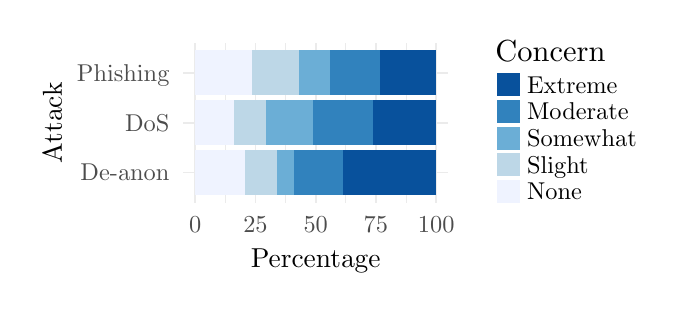
\begin{tikzpicture}[x=1pt,y=1pt]
\definecolor{fillColor}{RGB}{255,255,255}
\path[use as bounding box,fill=fillColor,fill opacity=0.00] (0,0) rectangle (231.26, 93.95);
\begin{scope}
\path[clip] ( 56.18, 30.77) rectangle (151.97, 88.45);
\definecolor{drawColor}{gray}{0.92}

\path[draw=drawColor,line width= 0.3pt,line join=round] ( 71.41, 30.77) --
	( 71.41, 88.45);

\path[draw=drawColor,line width= 0.3pt,line join=round] ( 93.18, 30.77) --
	( 93.18, 88.45);

\path[draw=drawColor,line width= 0.3pt,line join=round] (114.95, 30.77) --
	(114.95, 88.45);

\path[draw=drawColor,line width= 0.3pt,line join=round] (136.72, 30.77) --
	(136.72, 88.45);

\path[draw=drawColor,line width= 0.6pt,line join=round] ( 56.18, 41.59) --
	(151.97, 41.59);

\path[draw=drawColor,line width= 0.6pt,line join=round] ( 56.18, 59.61) --
	(151.97, 59.61);

\path[draw=drawColor,line width= 0.6pt,line join=round] ( 56.18, 77.64) --
	(151.97, 77.64);

\path[draw=drawColor,line width= 0.6pt,line join=round] ( 60.53, 30.77) --
	( 60.53, 88.45);

\path[draw=drawColor,line width= 0.6pt,line join=round] ( 82.30, 30.77) --
	( 82.30, 88.45);

\path[draw=drawColor,line width= 0.6pt,line join=round] (104.07, 30.77) --
	(104.07, 88.45);

\path[draw=drawColor,line width= 0.6pt,line join=round] (125.84, 30.77) --
	(125.84, 88.45);

\path[draw=drawColor,line width= 0.6pt,line join=round] (147.61, 30.77) --
	(147.61, 88.45);
\definecolor{fillColor}{RGB}{239,243,255}

\path[fill=fillColor] ( 60.53, 33.48) rectangle ( 78.46, 49.70);
\definecolor{fillColor}{RGB}{189,215,231}

\path[fill=fillColor] ( 78.46, 33.48) rectangle ( 89.99, 49.70);
\definecolor{fillColor}{RGB}{107,174,214}

\path[fill=fillColor] ( 89.99, 33.48) rectangle ( 96.39, 49.70);
\definecolor{fillColor}{RGB}{49,130,189}

\path[fill=fillColor] ( 96.39, 33.48) rectangle (113.89, 49.70);
\definecolor{fillColor}{RGB}{8,81,156}

\path[fill=fillColor] (113.89, 33.48) rectangle (147.61, 49.70);
\definecolor{fillColor}{RGB}{239,243,255}

\path[fill=fillColor] ( 60.53, 51.50) rectangle ( 74.55, 67.72);
\definecolor{fillColor}{RGB}{189,215,231}

\path[fill=fillColor] ( 74.55, 51.50) rectangle ( 86.02, 67.72);
\definecolor{fillColor}{RGB}{107,174,214}

\path[fill=fillColor] ( 86.02, 51.50) rectangle (103.01, 67.72);
\definecolor{fillColor}{RGB}{49,130,189}

\path[fill=fillColor] (103.01, 51.50) rectangle (124.67, 67.72);
\definecolor{fillColor}{RGB}{8,81,156}

\path[fill=fillColor] (124.67, 51.50) rectangle (147.61, 67.72);
\definecolor{fillColor}{RGB}{239,243,255}

\path[fill=fillColor] ( 60.53, 69.53) rectangle ( 80.91, 85.75);
\definecolor{fillColor}{RGB}{189,215,231}

\path[fill=fillColor] ( 80.91, 69.53) rectangle ( 97.90, 85.75);
\definecolor{fillColor}{RGB}{107,174,214}

\path[fill=fillColor] ( 97.90, 69.53) rectangle (109.37, 85.75);
\definecolor{fillColor}{RGB}{49,130,189}

\path[fill=fillColor] (109.37, 69.53) rectangle (127.21, 85.75);
\definecolor{fillColor}{RGB}{8,81,156}

\path[fill=fillColor] (127.21, 69.53) rectangle (147.60, 85.75);
\end{scope}
\begin{scope}
\path[clip] (  0.00,  0.00) rectangle (231.26, 93.95);
\definecolor{drawColor}{gray}{0.30}

\node[text=drawColor,anchor=base east,inner sep=0pt, outer sep=0pt, scale=  0.88] at ( 51.23, 38.56) {De-anon};

\node[text=drawColor,anchor=base east,inner sep=0pt, outer sep=0pt, scale=  0.88] at ( 51.23, 56.58) {DoS};

\node[text=drawColor,anchor=base east,inner sep=0pt, outer sep=0pt, scale=  0.88] at ( 51.23, 74.61) {Phishing};
\end{scope}
\begin{scope}
\path[clip] (  0.00,  0.00) rectangle (231.26, 93.95);
\definecolor{drawColor}{gray}{0.30}

\node[text=drawColor,anchor=base,inner sep=0pt, outer sep=0pt, scale=  0.88] at ( 60.53, 19.76) {0};

\node[text=drawColor,anchor=base,inner sep=0pt, outer sep=0pt, scale=  0.88] at ( 82.30, 19.76) {25};

\node[text=drawColor,anchor=base,inner sep=0pt, outer sep=0pt, scale=  0.88] at (104.07, 19.76) {50};

\node[text=drawColor,anchor=base,inner sep=0pt, outer sep=0pt, scale=  0.88] at (125.84, 19.76) {75};

\node[text=drawColor,anchor=base,inner sep=0pt, outer sep=0pt, scale=  0.88] at (147.61, 19.76) {100};
\end{scope}
\begin{scope}
\path[clip] (  0.00,  0.00) rectangle (231.26, 93.95);
\definecolor{drawColor}{RGB}{0,0,0}

\node[text=drawColor,anchor=base,inner sep=0pt, outer sep=0pt, scale=  0.99] at (104.07,  7.44) {Percentage};
\end{scope}
\begin{scope}
\path[clip] (  0.00,  0.00) rectangle (231.26, 93.95);
\definecolor{drawColor}{RGB}{0,0,0}

\node[text=drawColor,rotate= 90.00,anchor=base,inner sep=0pt, outer sep=0pt, scale=  0.99] at ( 12.32, 59.61) {Attack};
\end{scope}
\begin{scope}
\path[clip] (  0.00,  0.00) rectangle (231.26, 93.95);
\definecolor{drawColor}{RGB}{0,0,0}

\node[text=drawColor,anchor=base west,inner sep=0pt, outer sep=0pt, scale=  1.10] at (169.04, 81.72) {Concern};
\end{scope}
\begin{scope}
\path[clip] (  0.00,  0.00) rectangle (231.26, 93.95);
\definecolor{fillColor}{RGB}{8,81,156}

\path[fill=fillColor] (169.75, 69.18) rectangle (177.96, 77.40);
\end{scope}
\begin{scope}
\path[clip] (  0.00,  0.00) rectangle (231.26, 93.95);
\definecolor{fillColor}{RGB}{49,130,189}

\path[fill=fillColor] (169.75, 59.55) rectangle (177.96, 67.76);
\end{scope}
\begin{scope}
\path[clip] (  0.00,  0.00) rectangle (231.26, 93.95);
\definecolor{fillColor}{RGB}{107,174,214}

\path[fill=fillColor] (169.75, 49.91) rectangle (177.96, 58.12);
\end{scope}
\begin{scope}
\path[clip] (  0.00,  0.00) rectangle (231.26, 93.95);
\definecolor{fillColor}{RGB}{189,215,231}

\path[fill=fillColor] (169.75, 40.27) rectangle (177.96, 48.49);
\end{scope}
\begin{scope}
\path[clip] (  0.00,  0.00) rectangle (231.26, 93.95);
\definecolor{fillColor}{RGB}{239,243,255}

\path[fill=fillColor] (169.75, 30.64) rectangle (177.96, 38.85);
\end{scope}
\begin{scope}
\path[clip] (  0.00,  0.00) rectangle (231.26, 93.95);
\definecolor{drawColor}{RGB}{0,0,0}

\node[text=drawColor,anchor=base west,inner sep=0pt, outer sep=0pt, scale=  0.88] at (180.48, 70.26) {Extreme};
\end{scope}
\begin{scope}
\path[clip] (  0.00,  0.00) rectangle (231.26, 93.95);
\definecolor{drawColor}{RGB}{0,0,0}

\node[text=drawColor,anchor=base west,inner sep=0pt, outer sep=0pt, scale=  0.88] at (180.48, 60.62) {Moderate};
\end{scope}
\begin{scope}
\path[clip] (  0.00,  0.00) rectangle (231.26, 93.95);
\definecolor{drawColor}{RGB}{0,0,0}

\node[text=drawColor,anchor=base west,inner sep=0pt, outer sep=0pt, scale=  0.88] at (180.48, 50.99) {Somewhat};
\end{scope}
\begin{scope}
\path[clip] (  0.00,  0.00) rectangle (231.26, 93.95);
\definecolor{drawColor}{RGB}{0,0,0}

\node[text=drawColor,anchor=base west,inner sep=0pt, outer sep=0pt, scale=  0.88] at (180.48, 41.35) {Slight};
\end{scope}
\begin{scope}
\path[clip] (  0.00,  0.00) rectangle (231.26, 93.95);
\definecolor{drawColor}{RGB}{0,0,0}

\node[text=drawColor,anchor=base west,inner sep=0pt, outer sep=0pt, scale=  0.88] at (180.48, 31.71) {None};
\end{scope}
\end{tikzpicture}
